\vspace*{-0.1cm}
\beforesec
\section{Discussion}
\label{sec:discussion}
\postsec
This section further analyzes the empirical phenomena we have observed so far.
We begin with the case where only the final linear layer is fine-tuned and predictions from the weight-space ensemble can be factored into the outputs of the zero-shot and fine-tuned model.
Next, we connect our observations regarding end-to-end fine-tuning with earlier work on the phenomenology of deep learning.%
\vspace*{-0.1cm}
\beforesec
\subsection{Zero-shot and fine-tuned models are complementary}
\label{sec:decomposing}
\postsec


In this section, we find that the zero-shot and fine-tuned models have diverse predictions, both on reference and shifted distributions. Moreover, while the fine-tuned models are more confident on the reference distribution, the reverse is true under distribution shift.  

\smallpara{Zero-shot and fine-tuned models are diverse.}
\label{sec:diversity}
In certain cases, ensemble accuracy is correlated with diversity among the constituents \cite{kuncheva2003measures, gontijo2021no}.
If two models make coincident mistakes, so will their ensemble, and no benefit will be gained from combining them. 
Here, we explore two measures of diversity: {\it prediction diversity,} which measures the fraction of examples for which two classifiers disagree but one is correct; and {\it Centered Kernel Alignment Complement,}  the complement of CKA \cite{kornblith2019similarity}. 
Additional diversity measures and details are provided in Appendix \ref{sec:diversity_defs}.
In Figure \ref{fig:diversity_and_confidence} (left), we show that the zero-shot and fine-tuned models are diverse both on the reference and shifted distributions, despite sharing the same backbone. 
As a point of comparison, we include avg. diversity measures between two linear classifiers fine-tuned with random splits on half of 
ImageNet,\footnote{Two linear classifiers fine-tuned on the same data converge to similar solutions, resulting in negligible diversity. 
As a stronger baseline, we fine-tune classifiers on different subsets of ImageNet, with half of the data.} denoted in orange in Figure \ref{fig:diversity_and_confidence}.


\begin{figure*}
    \centering
    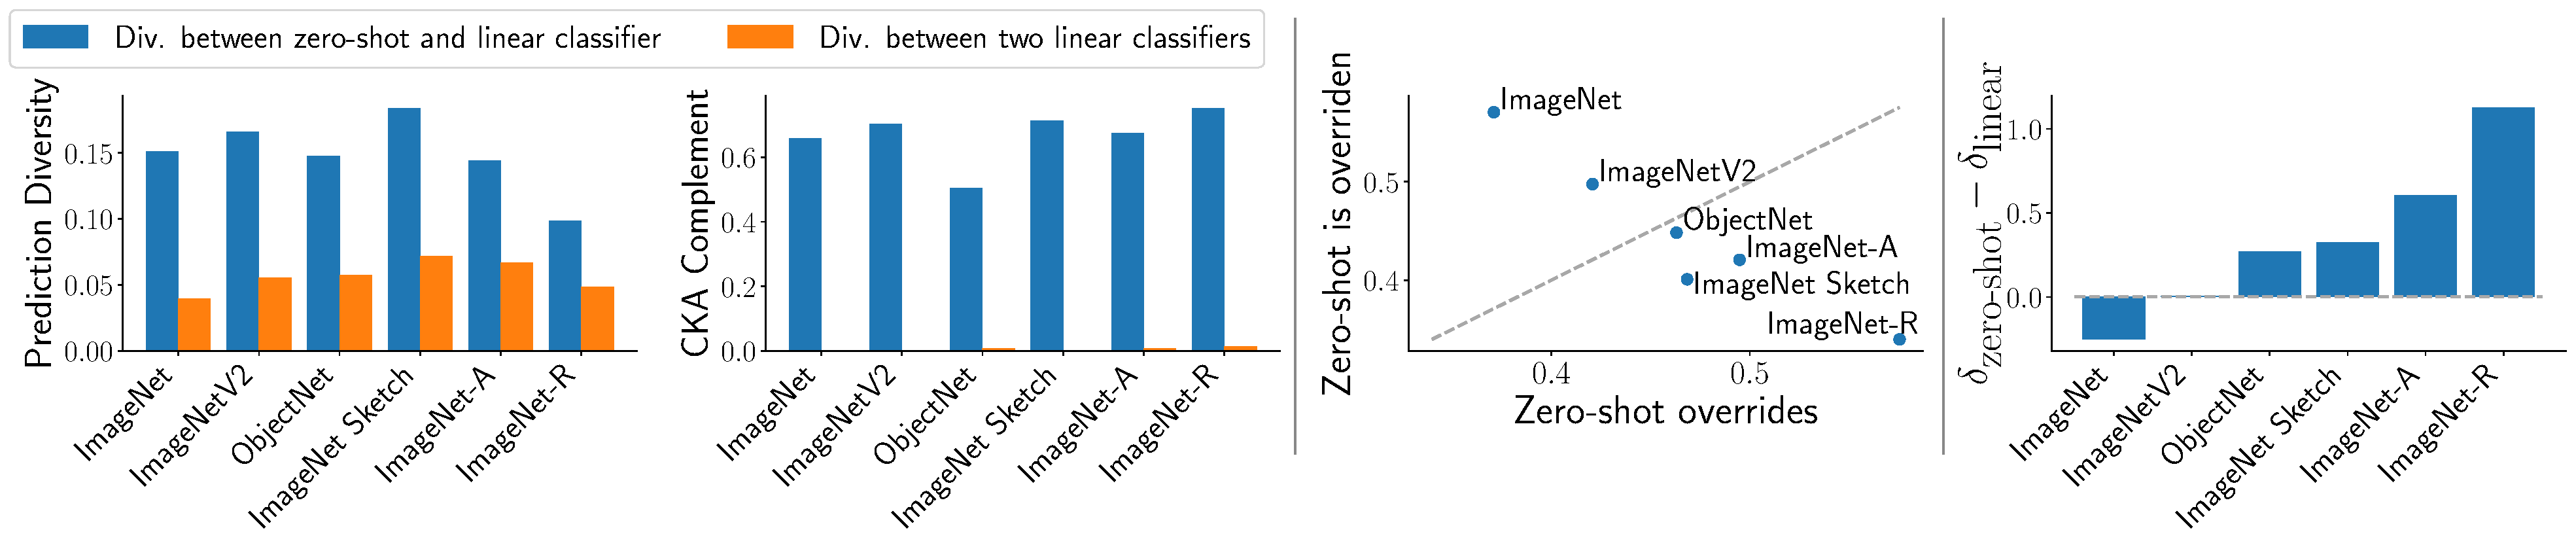
\includegraphics[width=\textwidth]{figures/diversity_and_confidence.pdf}
    \caption{\textbf{(Left)} Zero-shot and fine-tuned models exhibit diversity in their predictions. \textbf{(Middle)} On most distribution shifts, the zero-shot model overrides the linear classifier more than it is overridden. The reverse is true for ImageNet (reference). \textbf{(Right)} Similarly, zero-shot models are more confident under distribution shift, while the reverse is true on the reference distribution. The margin $\delta_f$ measures the average difference between the largest and second largest unormalized output for classifier $f$}
    \label{fig:diversity_and_confidence}
\end{figure*}

\smallpara{Models are more confident where they excel.}
In order for the ensemble model to be effective, it should leverage each model's expertise based on which distribution the data is from.
Here, we empirically show that this occurs on a number of datasets we consider.
First, we examine the cases where the models being ensembled disagree. 
We say the zero-shot model \textit{overrides} the fine-tuned model if their predictions disagree and the zero-shot prediction matches that of the weight-space ensemble. 
Similarly, if models disagree and the linear classifier prediction matches the ensemble, we say the zero-shot is \textit{overridden}.
Figure \ref{fig:diversity_and_confidence} (middle) shows the fraction of samples where the zero-shot model overrides and is overridden by the fine-tuned linear classifier for $\alpha{=}0.5$. 
Other than ImageNetV2, which was collected to closely reproduce ImageNet, the zero-shot model overrides the linear classifier more than it is overridden on the distribution shifts.

Additionally, we are interested in measuring model confidence. Recall that we are ensembling quantities before a softmax is applied, so we avoid criteria that use probability vectors, e.g., \citet{guo2017calibration}.
Instead, we consider the margin $\delta$ between the largest and second largest output of each classifier. 
Figure \ref{fig:diversity_and_confidence} (right) shows that the zero-shot model is more confident in its predictions under distribution shift, while the reverse is true on the reference distribution.
\beforesec
\subsection{An error landscape perspective}
\label{sec:landscape}
\postsec
We now turn to empirical phenomena we observe when weight-space ensembling \emph{all} layers in the network.
Specifically, this section formalizes our observations and details related phenomena. 
Recall that the weight-space ensemble of $\theta_0$ and $\theta_1$ is given by $f\mleft(x, (1-\alpha)\cdot\theta_0 + \alpha\cdot\theta_1 \mright)$ (Equation~\ref{eqn:wse}).

For a distribution $\mathcal{D}$ and model $f$, let $\mathsf{Acc}_{\mathcal{D}, f}(\theta)$ denote the expected accuracy of $f$ evaluated with parameters $\theta$ on distribution $\mathcal{D}$.


\begin{figure*}
    \centering
    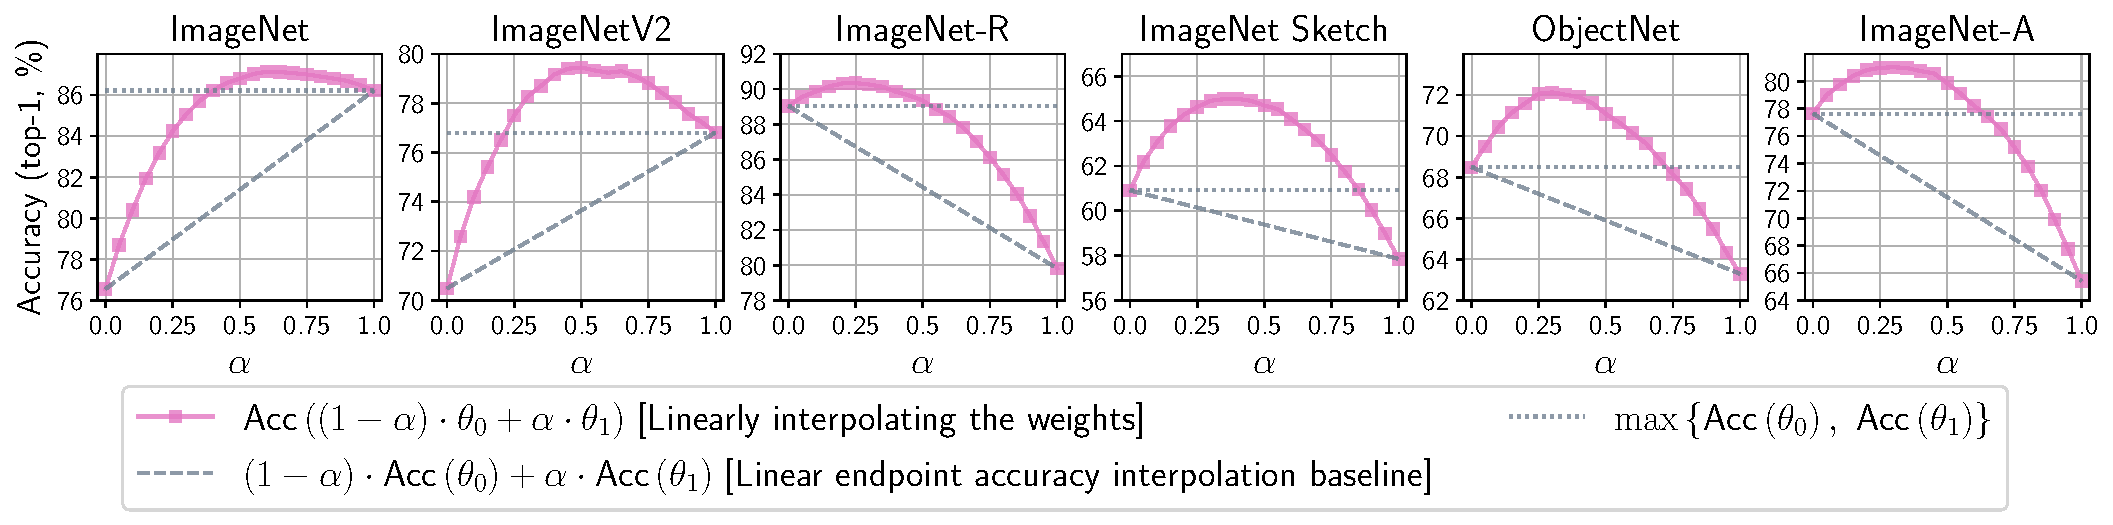
\includegraphics[width=\textwidth]{figures/figure_definition_small.pdf}
    \caption{On ImageNet and the main distribution shifts we consider, linearly interpolating between the weights of $\theta_0$ and $\theta_1$ exceeds the baseline of linearly interpolating the accuracies of the two models for all $\alpha$ (Observation 1). Moreover, there exists an $\alpha$ for which WiSE-FT outperforms both the zero-shot and fine-tuned models (Observation 2).}
    \label{fig:def}
\end{figure*}

\textbf{Observation 1:} As illustrated in Figure~\ref{fig:def}, on ImageNet and the five associated distribution shifts we consider
\begin{equation} \label{eq:base}
\mathsf{Acc}_{\mathcal{D}, f}\mleft((1-\alpha)\cdot \theta_0 +  \alpha \cdot \theta_1\mright)\ \geq \ (1-\alpha) \cdot \mathsf{Acc}_{\mathcal{D}, f}\mleft(\theta_0\mright) + \alpha \cdot \mathsf{Acc}_{\mathcal{D}, f}\mleft(\theta_1\mright)
\end{equation}
for all $\alpha \in [0,1]$.

Note that equation~\ref{eq:base} uses the baseline of linearly interpolating between the accuracies of the two endpoints, 
which is always achievable by using weights
$\theta_1$ with probability $\alpha$ and using model $\theta_0$ otherwise.
In the case where the accuracy of both endpoints are similar,
Equation~\ref{eq:base} is equivalent to the definition of Linear Mode Connectivity of \citet{frankle2020linear}.




To assist in contextualizing Observation 1, we review related phenomena. Neural networks are nonlinear, hence weight-space ensembles only achieve good performance in exceptional cases---interpolating the weights of two networks trained from a random initialization results in no better accuracy than a random classifier \cite{frankle2020linear}. 
Linear mode connectivity has been observed by 
\citet{frankle2020linear}; \citet{izmailov2018averaging}  when part of the training trajectory is shared, and by \citet{neyshabur2020being} when two models are fine-tuned with a shared initialization.
In particular, the observations of \citet{neyshabur2020being} may elucidate why weight-space ensembles attain high 
accuracy in the setting we consider, as they suggest that fine-tuning remains in a region where solutions are connected by a linear path along which error remains low.
Instead of considering the weight-space ensemble of two fine-tuned models, we consider the weight-space ensemble of the 
\textit{pre-trained} and fine-tuned models. This is only possible for a pre-trained model capable of zero-shot inference such as CLIP. 


\textbf{Observation 2:} As illustrated by Figure~\ref{fig:def}, on ImageNet and the five associated distribution shifts we consider, weight-space ensembling (end-to-end) may outperform both the zero-shot and fine-tuned models, i.e., there exists an $\alpha$ for which $\mathsf{Acc}_{\mathcal{D}, f}\left((1-\alpha) \cdot \theta_0 +  \alpha \cdot \theta_1\right) \ \geq \ \max\left\{  \mathsf{Acc}_{\mathcal{D}, f}\left(\theta_0\right) ,  \ \mathsf{Acc}_{\mathcal{D}, f}\left(\theta_1\right) \right\}$.

We are not the first to observe that when interpolating between models, the accuracy of models along the path may exceed that of either endpoint \cite{izmailov2018averaging, neyshabur2020being, pmlr-v139-wortsman21a}. \citet{neyshabur2020being}
conjecture that interpolation could produce solutions closer to the true center of a basin. 
In contrast to \citet{neyshabur2020being}, we interpolate between models which observe different data.










